\documentclass{article}
\usepackage[utf8]{inputenc}
\usepackage[spanish]{babel}
\usepackage{listings}
\usepackage{graphicx}
\graphicspath{ {images/} }
\usepackage{cite}

\begin{document}

\begin{titlepage}
    \begin{center}
        \vspace*{0cm}
            
        \Huge
        \textbf{Parcial 1}
            
        \vspace{0.5cm}
        \LARGE
        Informa2 S.A.S.
            
        \vspace{5cm}
            
        \textbf{David Agudelo Ochoa}
        
        \vspace{0.5cm}
        
        \textbf{Juan Pablo Cruz Gómez}
        
        \vspace{0.5cm}
        
        \textbf{Erika Dayana León Quiroga}
            
        \vfill
            
        \vspace{0.8cm}
            
        \Large
        Despartamento de Ingeniería Electrónica y Telecomunicaciones\\
        Universidad de Antioquia\\
        Medellín\\
        Marzo de 2021
            
    \end{center}
\end{titlepage}

\tableofcontents
\newpage
\section{Sección introductoria}\label{intro}
Este informe se hace con la intención de mostrar la solución de un problema cotidiano mediante el uso de  estructuras de programación, tipos de datos, funciones, arreglos y apuntadores usados en el lenguaje C++, además de introducir los conocimientos adquiridos sobre el Arduino, y lograr trabajar con estas dos herramientas para mostrar la propuesta implementada en el software de simulación de circuitos Tinkercad.

\section{Análisis del problema y consideraciones} \label{contenido}
En este problema, haciendo uso de tinkercad, se pide realizar la simulación de un circuito que controle un sistema compuesto por 64 LEDs (8 filas por 8 columnas) con ayuda de un arduino y la cantidad de circuitos integrados de registro de desplazamiento 74HC595 necesarios para su óptimo funcionamiento. El sistema compuesto por LEDs le mostrará al usuario el patrón de un caracter que él desee observar, el usuario podrá escribir palabras y el sistema se encargará de mostrar letra por letra, éstas separadas por un delay que el usuario escogerá a su gusto.
\subsection{Consideraciones iniciales}
Se debe tener en cuenta, según las restricciones, que se podrán usar máximo siete pines digitales del Arduino, se usarán dos circuitos integrados, cada uno de estos necesita tres pines digitales, uno de ellos controla las ocho filas y el otro las ocho columnas en el sistema compuesto por 64 LEDs. El pin sobrante, llamado Shift Register Clear, podrá ser utilizado como reset de la matriz de LEDs.

También es posible citar libros \cite{dirac} o documentos en línea \cite{knuthwebsite}.\\\\
Revisar en la última sección el formato de las referencias en IEEE.

\subsection{Incluir código en el documento}
%
A continuación, se presenta el código \ref{codigo_ejemplo}, que nos permite incluir en el informe partes de programa que requieran una explicación adicional.
\begin{lstlisting}[language=C++, label=codigo_ejemplo]
// Programa desarrollado, compilado y ejecutado en https://www.onlinegdb.com
#include <iostream>

/*
 * Esto es un comentario de varias lineas
 */

// Comentario de una sola linea

#define N 10

using namespace std;

int main()
{
    
    for( int i = 0 ; i < N ; i++ ){
        
        if( !(i % 2) )
            cout << " El valor de i es -> " << i << endl;
    }
    
    return 0;
}

//Resultado programa

/*
El valor de i es -> 0
El valor de i es -> 2
El valor de i es -> 4
El valor de i es -> 6
El valor de i es -> 8
*/
\end{lstlisting}
En la sección \ref{imagenes}, se presentará como añadir ilustraciones al texto.

\section{Tareas para el desarrollo del problema} \label{imagenes}
\begin{enumerate}
  \item Desarrollar una función para encender un led en una posición determinada, de esta forma se dará el primer paso para la creación de patrones complejos.
  \item Hacer una biblioteca de caracteres (Una función para cada caracter).
  \item Enlazar la biblioteca con el monitor serial mediante la función imagen, o sea, la entrada del usuario.
  \item Hacer el manual de usuario. Se incluirá la biblioteca de letras, números, caracteres comunes y caracteres especiales.
  \item Crear una función llamada Publik que le permite al usuario observar la secuencia de patrones con un delay asignado por el mismo usuario.
\end{enumerate}


\section{Algoritmo implementado} \label{imagenes}
\section{Problemas durante el desarrollo del desafío} \label{imagenes}
\section{Evolución del algoritmo} \label{imagenes}

\section{Inclusión de imágenes} \label{imagenes}

En la Figura (\ref{fig:montaje1}), se presenta el primer montaje del circuito. 

\begin{figure}[h]
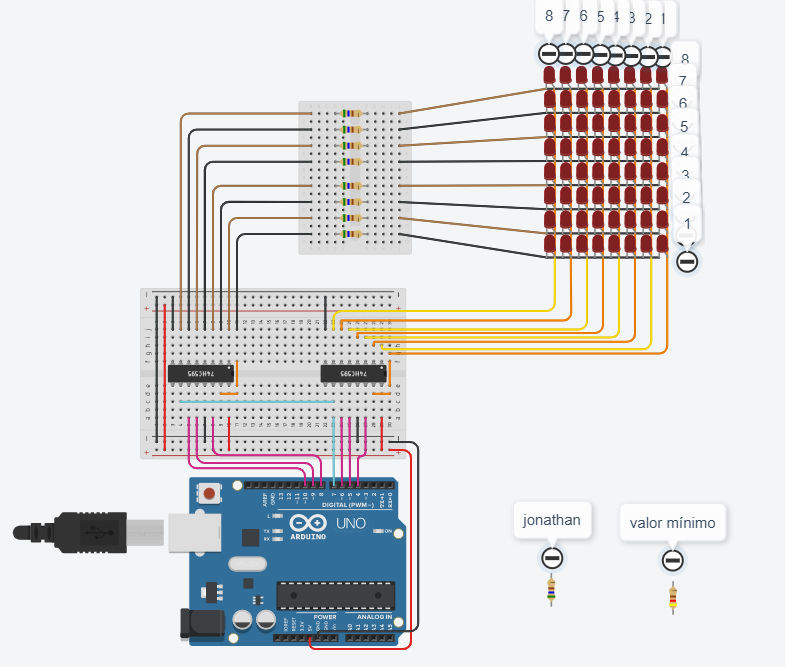
\includegraphics[width=16cm]{montaje1.png}
\centering
\caption{Primer montaje del circuito en Tinkercad}
\label{fig:montaje1}
\end{figure}

Las secciones (\ref{intro}), (\ref{contenido}) y (\ref{imagenes}) dependen del estilo del documento.

\bibliographystyle{IEEEtran}
\bibliography{references}

\end{document}
